\documentclass[10pt]{beamer}

%%%%%%%%%%%%%%%%%%%%%%%%%
%   Options for notes   %
%%%%%%%%%%%%%%%%%%%%%%%%%
% \setbeamertemplate{note page}[plain]
% \setbeameroption{show notes}
% \setbeameroption{show notes on second screen}
% \setbeameroption{show only notes}
% \setbeameroption{show only slides with notes}

\input{preamble}
\usepackage[ruled,vlined,linesnumbered]{algorithm2e}
% \algnewcommand\algorithmicinitialize{\textbf{initialize: }}
% \algnewcommand{\Initialize}[1]{\State \algorithmicinitialize #1}

%     presenter info    %
%%%%%%%%%%%%%%%%%%%%%%%%%
\author{
Xiaocheng ZHOU
}
\title{
Diffusion Models \& PRESCIENT
}
\subtitle{
Introduction to Diffusion Models\cite{guoDiffusionModelsBioinformatics2024,yangDiffusionModelsComprehensive2023a,pml2Book} \& an Related
Application in Development Biology\cite{hashimotoLearningPopulationlevelDiffusions2016,yeoGenerativeModelingSinglecell2021}
}
\date{Oct. 18, 2024}
\institute{
Journal Club
}

\begin{document}

% \kaishu
\begin{frame}
    \titlepage
    % \begin{figure}[htpb]
    %     \begin{center}
    %         
\includegraphics[width=0.2\linewidth]{pic/CUHKSZ-Logo.pdf}
    %     \end{center}
    % \end{figure}
\end{frame}

\section{Diffusion models: the basics}

\begin{frame}{Introduction to Diffusion models}
    The recent popular diffusion models are a family of probabilistic generative models:
    \begin{enumerate}
        \item progressively destruct data by injecting noise
        \item learn to reverse this process for sample reconstruction/generation
    \end{enumerate}
    
    The reverse process offers a flexible framework for modeling complex data distributions. 
    \begin{figure}[htpb]
        \centering
        
\includegraphics[width=0.8\linewidth]{20241018-Diffusion/figs/diffusion_overview.png}
        \caption{Diffusion models smoothly perturb data by adding noise and then reverse this process to generate new data from noise. The estimated score function is a gradient pointing to the directions of data with higher likelihood and less noise.} 
        \label{fig:diffusion_overview}
    \end{figure}

\end{frame}


\note[enumerate]{
    \item construct a series of training data from real data to noise following a simple distribution
    \item generates novel data from a simple prior distribution
}{}


\subsection{Denoising Diffusion Probabilistic Models (DDPMs)}

\subsubsection{Forward \& backward processes}

\begin{frame}{DDPM --- \normalsize Forward process}
    Given a real data distribution $\bm{x}_0\sim q(\bm{x}_0)$, incrementally transform it into a sequence of disturbed data 
    by a transition kernel $\bm{x}_t\sim q(\bm{x}_t\mid\bm{x}_{t-1})$ for $t=1,\cdots,T$
    \begin{gather}
        q(\bm{x}_t\mid\bm{x}_{t-1}) = \mathcal{N}(\bm{x}_t;\sqrt{1-\beta_t}\bm{x}_{t-1}, \beta_t\mathbf{I}),~\beta_t\in (0,1)~\text{known}\label{eq:ddpm}
    \end{gather}
    and finally into a tractable prior distribution.
    \begin{gather*}
        q(\bm{x}_t\mid\bm{x}_0) = \mathcal{N}(\bm{x}_t;\sqrt{\Bar{\alpha}_t}\bm{x}_0,(1-\Bar{\alpha}_t)\mathbf{I}),\\
        \alpha_t := 1-\beta_t,~\Bar{\alpha}_t:=\prod_{s=0}^t\alpha_s \to 0\\
        \implies q(\bm{x}_T\mid \bm{x}_0) \approx \mathcal{N}(\bm{x}_T;\bm{0},\mathbf{I})
    \end{gather*}
    Intuitively speaking, this forward process slowly injects noise into data until all structures are lost. 
\end{frame}

\note[enumerate]{
    \item The motivation is similar with VAE.
}{}



\begin{frame}{DDPM --- \normalsize Backward process}
    \begin{itemize}
        \item If original real data $\bm{x}_0$ is known, then the backward transition can be derived by conditional MVN of $q(\bm{x}_t\mid\bm{x}_{t-1})$ and $q(\bm{x}_t\mid\bm{x}_0)$,
        \begin{align*}
            \implies q(\bm{x}_{t-1}\mid\bm{x}_t,\bm{x}_0) & = \frac{q(\bm{x}_t\mid\bm{x}_{t-1})q(\bm{x}_{t-1}\mid\bm{x}_0)}{q(\bm{x}_t\mid\bm{x}_0)}  \\
            & = \mathcal{N}(\bm{x}_{t-1};\Tilde{\bm{\mu}}_t(\bm{x}_t,\bm{x}_0),\Tilde{\beta}_t\mathbf{I})
        \end{align*}

        \item Otherwise, a learnable Markov chain is parameterized by Neural Network and expected to gradually denoise from the prior distribution
        \begin{gather}
            p(\bm{x}_T)=\mathcal{N}(\bm{x}_T;\bm{0},\mathbf{I}), \notag\\
            \textcolor{blue}{p_{\bm{\theta}}}(\bm{x}_{t-1}\mid\bm{x}_{t})=\mathcal{N}(\bm{x}_{t-1};\textcolor{blue}{\mu_{\bm{\theta}}}(\bm{x}_t,t),\textcolor{blue}{{\Sigma}_{\bm{\theta}}}(\bm{x}_t,t)), \quad t=T,\cdots,1. \label{eq:learnableddpm}
        \end{gather}
        \textit{\textcolor{gray}{Usually, the variance is predefined as $\Tilde{\beta}_t\mathbf{I}$ or fixed $\sigma_t^2\mathbf{I}$.}}
    \end{itemize}
\end{frame}


\subsubsection{Training objective derivation}

\begin{frame}{DDPM --- \normalsize Training objective (ELBO)}
    We have two perspectives, that can be proven to be equivalent:
    \begin{enumerate}
        \item Maximize the likelihood $\textcolor{blue}{p_{\bm{\theta}}}(\bm{x}_0)$
        \item Minimize the distances between $q(\bm{x}_{t-1}\mid\bm{x}_t,\bm{x}_0)$ and $\textcolor{blue}{p_{\bm{\theta}}}(\bm{x}_{t-1}\mid\bm{x}_{t})$
    \end{enumerate}
    \bigskip
    First step: derive the ELBO like VAE (regard all the noisy samples $\bm{x}_{1:T}$ as a whole)
    \begin{align*}
        \log\textcolor{blue}{p_{\bm{\theta}}}(\bm{x}_0)
        & = \log\left[
            \int\textcolor{blue}{p_{\bm{\theta}}}(\bm{x}_{0,1:T})d\bm{x}_{1:T}
        \right] \\
        & = \log \mathbb{E}_{q(\bm{x}_{1:T}\mid \bm{x}_0)}\left[
            \frac{\textcolor{blue}{p_{\bm{\theta}}}(\bm{x}_{0,1:T})}{q(\bm{x}_{1:T}\mid \bm{x}_0)}
        \right] \\
        & \geq \underbrace{\mathbb{E}_{q(\bm{x}_{1:T}\mid \bm{x}_0)} \log \frac{\textcolor{blue}{p_{\bm{\theta}}}(\bm{x}_{0,1:T})}{q(\bm{x}_{1:T}\mid \bm{x}_0)}}_{=:\text{\L}(\bm{x}_0)\quad(\text{ELBO})}
    \end{align*}
\end{frame}


\begin{frame}{DDPM --- \normalsize Training objective (Series of $\infdiv{q(\cdot)}{\textcolor{blue}{p_{\bm{\theta}}}(\cdot)}$)}
    Then the ELBO can be decomposed into the two terms to compare
    {\footnotesize\begin{align*}
        \text{\L}(\bm{x}_0) 
        & = \mathbb{E}_{q(\bm{x}_{1:T}\mid \bm{x}_0)} \left[
            \log \frac{\textcolor{blue}{p_{\bm{\theta}}}(\bm{x}_{0,1:T})}{q(\bm{x}_{1:T}\mid \bm{x}_0)}
        \right] \\
        & = \mathbb{E}_{q(\bm{x}_{1:T}\mid \bm{x}_0)}\left[
        \log p(\bm{x}_T) + \sum_{t=1}^T\log\frac{\textcolor{blue}{p_{\bm{\theta}}}(\bm{x}_{t-1}\mid \bm{x}_t)}{q(\bm{x}_t\mid \bm{x}_{t-1})}
    \right] \\
        & = \mathbb{E}_{q(\bm{x}_{1:T}\mid\bm{x}_0)} \left[
            \log\frac{p(\bm{x}_T)}{q(\bm{x}_T\mid \bm{x}_0)} 
            + \sum_{t=2}^T\frac{\textcolor{blue}{p_{\bm{\theta}}}(\bm{x}_{t-1}\mid \bm{x}_t)}{q(\bm{x}_{t-1}\mid\bm{x}_t,\bm{x}_0)}
            + \log \textcolor{blue}{p_{\bm{\theta}}}(\bm{x}_{0}\mid \bm{x}_1)
        \right]  \\
        & = -\underbrace{\infdiv{q(\bm{x}_{T}\mid\bm{x}_0)}{p(\bm{x}_T)}}_{L_T(\bm{x}_0)~\text{prior loss}} 
        - \sum_{t=2}^T \underbrace{\mathbb{E}_{q(\bm{x}_{t}\mid\bm{x}_0)} \infdiv{q(\bm{x}_{t-1}\mid\bm{x}_t,\bm{x}_0)}{\textcolor{blue}{p_{\bm{\theta}}}(\bm{x}_{t-1}\mid \bm{x}_t)}}_{L_{t-1}(\bm{x}_0)~\text{diffusion loss}} - \\
        & \quad \underbrace{- \mathbb{E}_{q(\bm{x}_1\mid\bm{x}_0)}\log \textcolor{blue}{p_{\bm{\theta}}}(\bm{x}_0\mid\bm{x}_1)}_{L_0(\bm{x}_0)~\text{reconstruction loss}} \\
        & = -\text{const} - \sum_{t=1}^T \underbrace{\mathbb{E}_{q(\bm{x}_{t}\mid\bm{x}_0)} \infdiv{q(\bm{x}_{t-1}\mid\bm{x}_t,\bm{x}_0)}{\textcolor{blue}{p_{\bm{\theta}}}(\bm{x}_{t-1}\mid \bm{x}_t)}}_{L_{t-1}(\bm{x}_0)~\text{diffusion loss}+\text{reconstruction loss}} \\
        & =: - \mathcal{L}(\bm{x}_0)
    \end{align*}}
\end{frame}

\begin{frame}{DDPM --- \normalsize Training objective ($L_2$ loss of noises)}
    Each of these $\infdiv{q(\cdot)}{\textcolor{blue}{p_{\bm{\theta}}}(\cdot)}$ terms can be computed directly as $\|\bm{\mu}_q - \bm{\mu}_{\textcolor{blue}{p_{\bm{\theta}}}}\|^2$ since both of them are Gaussian. Since the mean of reverse sampling $q(\bm{x}_{t-1}\mid\bm{x}_t,\bm{x}_0)$ can be written as 
    $\Tilde{\bm{\mu}}_t(\bm{x}_t,\bm{x}_0) = \frac{1}{\sqrt{\alpha_t}}\left(
        \bm{x}_t - \frac{\beta_t}{\sqrt{1-\bar{\alpha}_t}}\bm{\varepsilon}
    \right)
    $,
    we can learn the noise from input $\bm{x}_{t}$ instead of the mean of $\bm{x}_{t-1}$ denoising from $\bm{x}_{t}$, i.e.
    $\textcolor{blue}{\bm{\mu}_{\bm{\theta}}}(\bm{x}_t,t)
    = \frac{1}{\sqrt{\alpha_t}}\left(
        \bm{x}_t - \frac{\beta_t}{\sqrt{1-\bar{\alpha}_t}}\textcolor{blue}{\bm{\varepsilon}_{\bm{\theta}}}(\bm{x}_t,t)
    \right)$.
    {\small\begin{align*}
        \mathcal{L}_{t-1} & := \mathbb{E}_{q(\bm{x}_0)}L_{t-1}(\bm{x}_0) \notag \\
        & = \mathbb{E}_{q(\bm{x}_0)} \mathbb{E}_{q(\bm{x}_{t}\mid\bm{x}_0)} \infdiv{q(\bm{x}_{t-1}\mid\bm{x}_t,\bm{x}_0)}{\textcolor{blue}{p_{\bm{\theta}}}(\bm{x}_{t-1}\mid \bm{x}_t)} \notag \\
        & = \mathbb{E}_{\bm{x}_0\sim q(\bm{x}_0),\varepsilon\sim\mathcal{N}(\bm{0},\mathbf{I})}\bigg[
            \underbrace{\frac{\beta_t^2}{2\sigma_t^2\alpha_t(1-\bar{\alpha}_t)}}_{\lambda(t)}\bigg\|
                \bm{\varepsilon} - \textcolor{blue}{\bm{\varepsilon}_{\bm{\theta}}}\big(\underbrace{
                    \sqrt{\bar{\alpha}_t}\bm{x}_0 + \sqrt{1-\bar{\alpha}_t}\bm{\varepsilon}
                }_{\bm{x}_t}, t\big)
            \bigg\|^2
        \bigg],\label{eq:ddpmmseloss}
    \end{align*}}
    where $\lambda(t)$ is the weight for sampling each time point, and it is usually set $\lambda(t)\equiv 1$ in DDPM, then
    {\small\begin{gather}
        \mathcal{L}_\text{simple}
        = \mathbb{E}_{\bm{x}_0\sim q(\bm{x}_0),\varepsilon\sim\mathcal{N}(\bm{0},\mathbf{I}),t\sim\mathcal{U}\{1,\cdots,T\}}
        \bigg\|
            \bm{\varepsilon} - \textcolor{blue}{\bm{\varepsilon}_{\bm{\theta}}}\big(\underbrace{
                \sqrt{\bar{\alpha}_t}\bm{x}_0 + \sqrt{1-\bar{\alpha}_t}\bm{\varepsilon}
            }_{\bm{x}_t}, t\big)
        \bigg\|^2
    \end{gather}}
\end{frame}

\subsubsection{Samling from model}

\begin{frame}{DDPM --- \normalsize Sampling from the Trained Denoiser}
    Sampling new data is involved in the process of training and inference,
    we can implement it by sampling from noises according to Algorthm \ref{alg:ddpm}.
    
    \bigskip
    
    \begin{algorithm}[H]
        \SetAlgoLined
        \SetKwInOut{Input}{Input}
        \SetKwInOut{Output}{Output}
        \Input{An estimated noise function $\textcolor{blue}{\bm{\varepsilon}_{\bm{\theta}}(\bm{x},t)}$}
        \Input{A series of noise schedule $\{\sigma_t\}_{t=1}^{T}$}
        \Output{A valid sample $\bm{x}_0 \sim \textcolor{blue}{p_{\bm{\theta}}(\bm{x}_0)}$ }
        \BlankLine
        
        $\bm{x}_T \gets \mathcal{N}(\bm{0},\mathbf{I})$ \\
        \For{$t = T$ to $1$}{
            $\bm{\varepsilon}_t \gets \mathcal{N}(\bm{0},\bm{I})$\\
            $\bm{x}_{t-1} \gets \frac{1}{\sqrt{\alpha_t}}\left(\bm{x}_t - \frac{1 - \alpha_t}{\sqrt{1-\bar{\alpha}_t}}\textcolor{blue}{\bm{\varepsilon}_{\bm{\theta}}}(\bm{x}_t,t)\right) + \sigma_t\bm{\varepsilon}_t$
        }
        return $\bm{x}_0$
        \caption{Sampling from DDPM model}
        \label{alg:ddpm}
    \end{algorithm}
\end{frame}


\subsection{Score-based Generative Models (SGMs)}

\subsubsection{Scoring Networks}

\begin{frame}{Scoring Networks --- \normalsize Score function}
    We can estimate $p_{\theta}(\bm{x})$ for $q(\bm{x}_0)$ of any real data distribution
    by estimating its score function $\textcolor{blue}{\bm{s}_{\bm{\theta}}}:=\nabla_{\bm{x}}\log p_{\theta}(\bm{x})$ since
    \begin{gather*}
        \forall~\text{p.d.f.}~p_{\theta}(\bm{x}),~\exists \mathcal{E}_{\theta}(\bm{x})\in \mathbb{R}~\text{s.t.}~p_{\theta}(\bm{x}) = \frac{\exp(-\mathcal{E}_{\theta}(\bm{x}))}{Z_{\theta}}\\
        \implies \nabla_{\bm{x}}\log p_{\theta}(\bm{x}) = -\nabla_{\bm{x}}\mathcal{E}_{\theta}(\bm{x})
    \end{gather*}
    where $Z_{\theta}=\int \exp(-\mathcal{E}_{\theta}(\bm{x}))d\bm{x}$. The objective function of the scoring network can be defined by Fisher divergence
    \begin{gather*}
    \mathbb{E}_{\bm{x}_0\sim q(\bm{x}_0)}\left\|
        \nabla_{\bm{x}_0}\log q(\bm{x}_0) - \textcolor{blue}{\bm{s}_{\bm{\theta}}}(\bm{x}_0)
    \right\|^2.
    \end{gather*}
    However, it can not be optimized directly since $\nabla_{\bm{x}_0}\log q(\bm{x}_0)$ is unknown.
    
    \medskip
    
    \begin{definition}[(Stein) Score]
        Given a p.d.f. $q(\bm{x})$, its score function is defined as the gradient of the log p.d.f. $\nabla_{\bm{x}}\log q(\bm{x})$. It is a vector field that points to directions along which the p.d.f. has the largest rate. 
    \end{definition}
\end{frame}

\subsubsection{Score matching}
\begin{frame}{SGM --- \normalsize Score matching \& Sampling around real data}
    The above estimation problem can be solved by score matching: 
    \begin{enumerate}
        \item sample perturbed data from a known distribution around the real data \textcolor{gray}{(to let the empirical $\hat{q}(\bm{x}_0)$ smoother)} 
        \item minimize the distances between the scores of these known distributions and the estimation.
    \end{enumerate}
    
    \bigskip
    
    Similar to DDPM, we can obtain a sequence of noisy data with incremental noise levels, 
    $0 < \sigma_1 < \sigma_2 < \cdots < \sigma_T$, \textcolor{gray}{\textit{(instead of defining each step})}
    from the original real data $\bm{x}_0$:
    \begin{gather}
        q(\bm{x}_t\mid\bm{x}_0) = \mathcal{N}(\bm{x}_t;\bm{x}_0,\sigma^2_t\mathbf{I}),~t=1,\cdots,T \label{eq:sgm}\\
        \implies q(\bm{x}_t) = \mathbb{E}_{q(\bm{x}_0)}q(\bm{x}_t\mid\bm{x}_0)~\text{known}\notag
    \end{gather}
\end{frame}

\begin{frame}{SGM --- \normalsize Training objective}
    The original objective can be defined as
    {\small\begin{align}
        \mathcal{L} 
        & \propto \mathbb{E}_{\bm{x}_t\sim q(\bm{x}_t),t\sim\mathcal{U}\{1,\cdots,T\}}
        \left[\lambda'(t)\left\|
            \nabla_{\bm{x}_t}\log q(\bm{x}_t) - \textcolor{blue}{\bm{s}_{\bm{\theta}}}(\bm{x}_t, t)
        \right\|^2\right] \notag\\
        & \propto \mathbb{E}_{\bm{x}_0\sim q(\bm{x}_0),\bm{x}_t\sim q(\bm{x}_t\mid\bm{x}_0),t\sim\mathcal{U}\{1,\cdots,T\}}
        \left[\lambda'(t)\left\|
            \nabla_{\bm{x}_t}\log q(\bm{x}_t\mid\bm{x}_0) - \textcolor{blue}{\bm{s}_{\bm{\theta}}}(\bm{x}_t, t)
        \right\|^2\right] \label{eq:sgmvarobj}\\
        & = \mathbb{E}_{\bm{x}_0\sim q(\bm{x}_0),\bm{x}_t\sim q(\bm{x}_t\mid\bm{x}_0),t\sim\mathcal{U}\{1,\cdots,T\}}
        \left[\lambda'(t)\left\|
            - \frac{\bm{x}_t - \bm{x}_0}{\sigma_t^2} - \textcolor{blue}{\bm{s}_{\bm{\theta}}}(\bm{x}_t, t)
        \right\|^2\right] \notag\\
        & = \mathbb{E}_{\bm{x}_0\sim q(\bm{x}_0),\bm{x}_t\sim q(\bm{x}_t\mid\bm{x}_0),t\sim\mathcal{U}\{1,\cdots,T\}}
        \big[\underbrace{\lambda'(t)\sigma_t^2}_{\lambda(t)}\big\|
            \underbrace{\bm{x}_t - \bm{x}_0}_{\bm{\varepsilon}} - 
            \underbrace{[- \sigma_t^2\textcolor{blue}{\bm{s}_{\bm{\theta}}}(\bm{x}_t, t)]}_{\textcolor{blue}{\bm{\varepsilon}_{\bm{\theta}}}(\bm{x}_t, t)}
        \big\|^2\big],\notag
    \end{align}}
    thus the training objectives of DDPMs and SGMs are equivalent if $\bm{\varepsilon}_{\bm{\theta}}(\bm{x}_t,t)=-\sigma_t^2\bm{s}_{\bm{\theta}}(\bm{x}_t,t)$ is set. \textcolor{gray}{\textit{The negative score represents the noise added at $\bm{x}_t$ to reduce log-likelihood/energy as shown in Figure \ref{fig:diffusion_overview}.}}
\end{frame}

\subsubsection{Samping from model}
\begin{frame}{SGM --- \normalsize Sampling from the scoring function}
    The annealed Langevin dynamics algorithm (MCMC procedure) is used 
    to sample $\bm{x}_t$ recursively from the score function.

    \smallskip

    {\small\begin{algorithm}[H]
        \SetAlgoLined
        \SetKwInOut{Input}{Input}
        \SetKwInOut{Output}{Output}
        \Input{An estimated score function $\textcolor{blue}{\bm{s}_{\bm{\theta}}(\bm{x},t)}$}
        \Input{Number of iterations per time $N\to\infty$}
        \Input{A series of step sizes $\{s_t\to 0\}_{t=0}^{T-1}$}
        \Output{A valid sample $\bm{x}_0^{(N)}\sim \textcolor{blue}{p_{\bm{\theta}}(\bm{x}_0)}$ }
        \BlankLine
    
        $\bm{x}_T^{(N)} \gets \mathcal{N}(\bm{0},\mathbf{I})$ \\
        \For{$t = T-1$ to $0$}{
            $\bm{x}_{t}^{(0)} = \bm{x}_{t+1}^{N}$\\
            \For{$i=0$ to $N-1$}{
                $\bm{\varepsilon}^{(i)} \gets \mathcal{N}(\bm{0},\bm{I})$\\
                $\bm{x}_t^{(i+1)} \gets \bm{x}_t^{(i)} + \frac{1}{2} s_t \textcolor{blue}{\bm{s}_{\bm{\theta}}}(\bm{x}_t^{(i)},t) + \sqrt{s_t}\bm{\varepsilon}^{(i)}$\\
            }
        }
        return $\bm{x}_0^{(N)}$
        \caption{Sampling from SGM model (ALD algorithm)}
    \end{algorithm}}
\end{frame}


\subsection{Score-based  Stochastic Differential Equations (Score SDEs)}

\subsubsection{From discrete to continuous}

\begin{frame}{Score SDE --- \normalsize Forward diffusion SDE}
    Consider a diffusion process where the noise level $\beta_t$ gets rewritten as $\beta(t)\Delta t$, 
    where $\Delta t$ is a step size:
    \begin{align*}
        \bm{x}_t & = \sqrt{1-\beta_t}\bm{x}_{t-1} + \sqrt{\beta_t}\bm{\varepsilon},~ \bm{\varepsilon}\sim\mathcal{N}(\bm{0},\mathbf{I}) \\
        \implies \bm{x}_t & = \sqrt{1-\beta(t)\Delta t}\bm{x}_{t-\Delta t} + \sqrt{\beta(t)\Delta t}\bm{\varepsilon} \\
       \textcolor{gray}{\text{(by Taylor)}} & \approx \bm{x}_{t-\Delta t} - \frac{\beta(t)\Delta t}{2}\bm{x}_{t-\Delta t} + \sqrt{\beta(t)\Delta t}\bm{\varepsilon},~\Delta t \to 0 \\
       \implies {d\bm{x}(t)} & = -\frac{1}{2}\beta(t)\bm{x}(t)dt + \sqrt{\beta(t)}d\bm{w}(t)
       \end{align*}
       \begin{gather}
        \implies d\bm{x}(t) = \underbrace{\bm{f}(\bm{x},t)}_\text{draft}dt + \underbrace{g(t)}_\text{diffusion}d\bm{w}(t),~t\in[0,T], \label{eq:diffusionsde}
    \end{gather}
    where $\bm{w}(t)$ represents a standard Wiener process\footnote{also called Brownian noise, definition: $\bm{w}(t)-\bm{w}(s)\sim\mathcal{N}(0, t-s)$, $\forall{0\leq s < t}$, thus $d\bm{w}(t)\sim \mathcal{N}(0,dt)$}.
\end{frame}

\begin{frame}{Score SDE --- \normalsize Special cases: DDPM \& SGM}
    The SDE corresponding to DDPMs is given by
    \begin{gather*}
        d\bm{x}(t) = -\frac{1}{2}\beta(t)\bm{x}(t)dt + \sqrt{\beta(t)}d\bm{w}(t),
    \end{gather*}
    where the draft term is proportional to $-\bm{x}(t)$, encouraging the process to \textbf{return to 0} (variance preserving). 
    
    \bigskip
    
    However, the SDE corresponding to SGMs has no draft to control the growth of noise (variance exploding), which is analogous to perturbing data with incremental noise levels to \textbf{totally random}.
    \begin{gather*}
        d\bm{x}(t) = 0 + \sqrt{\frac{d[\sigma^2(t)]}{dt}}d\bm{w}(t).
    \end{gather*}
\end{frame}

\subsubsection{Reverse, Objective, and Sampling}

\begin{frame}{SSDE --- \normalsize Reverse process}
    \begin{itemize}
        \item \textbf{Reverse process}: Eq. \eqref{eq:diffusionsde} can be reversed to get the following reverse-time SDE.
        \begin{gather}
            d\bm{x} = \big[
                \bm{f}(\bm{x},t) - g^2(t)\underbrace{\nabla_{\bm{x}}\log q_t(\bm{x})}_{\text{score}}
            \big]dt + g(t)d\Tilde{\bm{w}},
        \end{gather}
        where $\Tilde{\bm{w}}(t)$ is the reverse-time standard Wiener process\footnote{$\Tilde{\bm{w}}(t)\triangleq\bm{w}(T-t)$, $t\in[0,T]$} and $dt < 0$.
    \end{itemize}
    
    \bigskip
    
    \begin{figure}
        \centering
        
\includegraphics[width=0.6\linewidth]{20241018-Diffusion/figs/sde_schematic.jpg}
        \caption{Any SDE has a corresponding reverse SDE}
        \label{fig:sde_schematic}
    \end{figure}
\end{frame}

\begin{frame}{SSDE --- \normalsize Training objective \& Sampling from score function}
    \begin{itemize}
        \item \textbf{Training objective}: similar to the estimation in SGMs, but continuous time $t$ is sampled.
        {\footnotesize\begin{gather}
            \mathcal{L} = \\
            \mathbb{E}_{\bm{x}(0)\sim q(\bm{x}(0)),\bm{x}(t)\sim q(\bm{x}(t)\mid\bm{x}(0)),\textcolor{purple}{t\sim\mathcal{U}[0,T]}}\notag
            \left[\lambda(t)\left\|
                \nabla_{\bm{x}(t)}\log q(\bm{x}(t)\mid\bm{x}(0)) - 
                \textcolor{blue}{\bm{s}_{\bm{\theta}}}(\bm{x}(t), t)
            \right\|^2\right]
        \end{gather}}

        \smallskip

        \item \textbf{Sampling}: Apply the Euler-Maruyama integration over time to obtain a valid $\bm{x}_0$.
        {\footnotesize\begin{gather}
            \bm{x}(t-\Delta t)
            = \bm{x}(t) + \left[
                \bm{f}(\bm{x}(t),t) - g^2(t)\textcolor{blue}{\bm{s}_{\bm{\theta}}}(\bm{x}(t),t)
            \right]\Delta t + g(t)\sqrt{\Delta t} \mathcal{N}(\bm{0},\mathbf{I})
        \end{gather}}
    \end{itemize}
\end{frame}

\begin{frame}{Short summary of diffusion model}
    The key idea behind diffusion models is to 
    \begin{enumerate}
        \item progressively destroy data by injecting noise, transforming real data into noisy data following a simple distribution, and then
        \item \textbf{learns to reverse this process}, enabling novel data generation from a simple prior distribution.
    \end{enumerate}

    \bigskip

    The improvement of the diffusion model focuses on 
    \begin{enumerate}
        \item Sampling acceleration: distillations, training schedule optimization, training-free acceleration, and integration of diffusion models with faster generative models.
        \item Diffusion process design: shift from Euclidean space to another space.
        \item Likelihood optimization: learning with log-likelihood is challenging for continuous-time diffusion models.
    \end{enumerate}
\end{frame}


\section{An Application in Development Biology}

\subsection{Introduction}


\begin{frame}{Preface}
    \begin{figure}
        \centering
        
\includegraphics[width=0.9\linewidth]{20241018-Diffusion/figs/PRESEIENT_title.png}
        \caption{Paper to be presented. Published in 2021, learning the draft function from time-resolved RNA-seq data}
        \label{fig:PRESEIENT_title}
    \end{figure}
\end{frame}

\begin{frame}{Introduction --- \normalsize Challenges in studying development trajectory}
    Modeling the developmental trajectory is essential to improving our understanding of how cells are driven to transient and terminal states in vivo and to enable the manipulation of cell fates in vitro.
    
    \medskip
    
    scRNA-seq can only provide \textbf{population snapshots at multiple development stages} instead of tracing cell lineage for a specific cell, even though it measures gene expression at a single-cell level.

    \bigskip
    
    \begin{figure}
        \centering
        
\includegraphics[width=0.8\linewidth]{20241018-Diffusion/figs/celldiff.png}
        \caption{Embryo stem cells’ development paths, processes regulated by transcription regulators expressed or alternated along trajectory}
        \label{fig:celldiff}
    \end{figure}

\end{frame}


\subsection{Method}

\begin{frame}{Method --- \normalsize Overview of modeling and validation}
    PRESCIENT applies a diffusion-based approach to model the \textbf{global potential function of a time series} by fitting only well-mixed, cross-sectional observations at several time points.

    \medskip
    
    Once fitted, the potential function can 
    \begin{enumerate}
        \item simulate trajectories for the cells unobserved during training and
        \item predict cell fate bias given its initial state with/without computationally perturbed gene expression profiles.
    \end{enumerate} 


    \begin{figure}[htpb]
        \centering
        
\includegraphics[width=0.6\linewidth]{20241018-Diffusion/figs/PRESEIENT_overview_datatrain.png}
        \caption{Overview of the diffusion-based model and recursive training strategy}
        \label{fig:PRESEIENT_overview_datatrain}
    \end{figure}
\end{frame}


\begin{frame}{Method --- \normalsize Population-level scRNA-seq Snapshots}
    Available scRNA-seq datasets are snapshots of different development stages, 
    which can be formulated as 
    \begin{align*}
        \left\{[\bm{x}(t)]_j\right\}_{j=1}^{m_t} \sim \rho(\bm{x},t):= P(\bm{X}(t)=\bm{x}),~t\in\mathcal{T}:=\{0,t_1,\cdots,t_n\}
    \end{align*}
    \begin{itemize}
        \item $[\bm{x}(t)]_j$: expression profile of cell $i$ collected at time $t$
        \item $\rho(\bm{x},t)$: distribution of expression profile at time $t$
        \item $\{0,t_1,\cdots,t_n\}$: all considered time points of experiments
        \item $m_t$: number of cells collected at time $t$
    \end{itemize}

    \bigskip

    \begin{figure}
        \centering
        
\includegraphics[width=0.6\linewidth]{20241018-Diffusion/figs/nontracing_seq_barcode.png}
        \caption{Time-resolved snapshots of scRNA-seq cells. We only know the population-level data but do not trace a cell.}
        \label{fig:nontracing_seq_barcode}
    \end{figure}
\end{frame}


\begin{frame}{Method --- \normalsize Diffusion-based Model}
    Diffusion model considered here is given by:
    \begin{gather}
        \bm{x}(t+\Delta t) = \bm{x}(t) + \bm{f}(\bm{x}(t))\Delta t + \sqrt{2\sigma^2\Delta t}\bm{\varepsilon}(t), \label{eq:diffusionsdepaper}
    \end{gather}
    \begin{itemize}
        \item $\textcolor{purple}{\bm{f}(\bm{x}(t))}\Delta t$: drift term, representing the evolution of a cell's RNA expression $\bm{x}$ at time $t$ during the following period $\Delta t$.
        \item $\sqrt{\sigma^2\Delta t}\bm{\varepsilon}$: diffusion/noise term, capturing the stochasticity, $\sigma^2$ given.
    \end{itemize}
    
    \medskip
    
    \begin{figure}[htpb]
        \centering
        \begin{subfigure}[b]{0.25\textwidth}
            \centering
            
\includegraphics[width=\textwidth]{20241018-Diffusion/figs/Waddington-epigenetic-landscape.jpg}
            \caption{Waddington's epigenetic landscape. The cells differentiate from high potential to low potential.}
            \label{fig:epigenetic-landscape}
        \end{subfigure}
        \quad
        \begin{subfigure}[b]{0.25\textwidth}
            \centering
            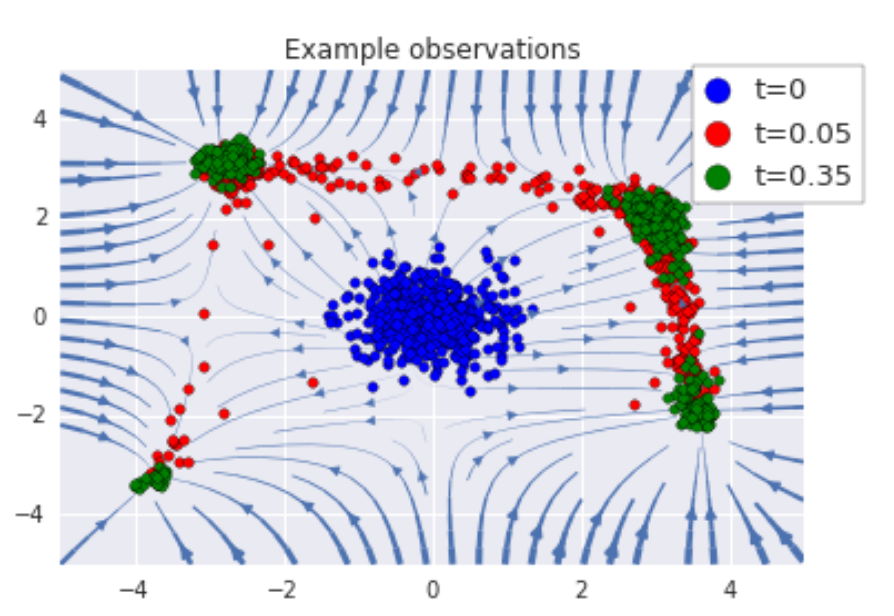
\includegraphics[width=\textwidth]{figs/potential_field.png}
            \caption{We observe samples (colored points) drawn from the process at different times. The goal is to infer the dynamics (\textcolor{blue}{$\rightarrow$}), i.e. $\bm{f}(\bm{x})$, the force acting on the cell given its current state $\bm{x}(t)$}
            \label{fig:potential_field}
        \end{subfigure}
        \caption{Estimate the draft function from time-resolved population-level data}
        \label{fig:differentiation-field}
    \end{figure}

\end{frame}


\begin{frame}{Method --- \normalsize Estimation of drift function from the snapshots}
    \small
    This model uses a 2-layer MLP $\textcolor{blue}{\Psi_{\bm{\theta}}}$ to parameterize the potential function,
    then the training objective for estimating the draft function is given by\cite{hashimotoLearningPopulationlevelDiffusions2016}  
    \begin{gather}
        \mathcal{L}(\bm{\theta}) 
        = \sum_{i=1}^n W_2^2(\hat{\rho}(\bm{X},t_i),\textcolor{blue}{\rho_{\Psi_{\bm{\theta}}}}(\bm{X},t_i))
        + \tau\sum_{j=1}^{m_n}\frac{\textcolor{blue}{\Psi_{\bm{\theta}}}(\bm{x}_j)}{\sigma^2}
    \end{gather}

    \begin{itemize}
        \item First term: distance between empirical and predicted distributions over all time points
        \begin{itemize}
            \item $W_p$: p-norm Wasserstein distances between two distributions
            \item $\hat{\rho}(\bm{X},t_i)$: $\{[\bm{x}(t_i)]_j\}_{j=1}^{m_i}$ and $\textcolor{blue}{\rho_{\Psi_{\bm{\theta}}}}(\bm{X},t_i))$: $\{\textcolor{blue}{[\hat{\bm{x}}(t_i)]_{j'}}\}_{j'=1}^{m'_i}$, the predictions sampled from the following forward stochastic process:
            {\small\begin{gather*}
                \textcolor{blue}{\hat{\bm{x}}(t_i)} = \textcolor{blue}{\hat{\bm{x}}(t_{i-1})} + \textcolor{blue}{\bm{f}_{\bm{\theta}}}(\textcolor{blue}{\hat{\bm{x}}(t_{i-1})})(t_i-t_{i-1}) + \sqrt{\sigma^2(t_i-t_{i-1})} \bm{\varepsilon}(t_i)
            \end{gather*}}
            \item $\textcolor{blue}{\bm{f}_{\bm{\theta}}} = - \nabla_{\bm{x}}\textcolor{blue}{\Psi_{\bm{\theta}}}$ by automatical differentiation
        \end{itemize}
        
        \item Second term: the theory in the ICML paper\cite{hashimotoLearningPopulationlevelDiffusions2016} proved that if the distribution at final time $t_n$ is \textit{well-mixed}, then true $\Psi$ can be recovered well. 
        \item $\tau$: regularization parameter to combine these two objects
    \end{itemize}

\end{frame}

\note[enumerate]{
    \item So far, this model is similar to the previously presented OT-based paper, 
    \item mapping between adjacent time points, but implicitly learning the optimal mapping between
    \item the actual measurements and generated predictions at the same time points in a series
    with the assumption of final dynamic equilibrium.
}{}

\begin{frame}{Method --- \normalsize Incorporating Cell Proliferation: re-weight OT}
    \small
    Computing the Wasserstein distance involves solving the optimal transport problem
    \begin{align}
        \min_{\mathbf{P},\textcolor{blue}{\mathbf{C}}}~& \sum_{j,j'}P_{j,j'}C_{j,j'} \\
        \text{s.t.}~ & \sum_{j'=1}^{m'}P_{j,j'} = \alpha_j,~ \sum_{j=1}^{m}P_{j,j'} = \beta_{j'} \\
        & P_{i,j} \geq 0,~\forall j=1,\cdots,m,~j'=1,\cdots,m' 
    \end{align}
    \begin{itemize}
        \item $P_{j,j'}$: transport plan between $\bm{x}_j$ and $\textcolor{blue}{\hat{\bm{x}}_{j'}}$
        \item $\textcolor{blue}{C_{j,j'}}$: cost transporting between $\bm{x}_j$ and $\textcolor{blue}{\hat{\bm{x}}_{j'}}$, $\|\bm{x}_j-\textcolor{blue}{\hat{\bm{x}}_{j'}}\|_2^2$ here \textcolor{gray}{\textit{(corresponding to $W_2$)}}
        \item $\alpha_j$: probability mass of real profile $\bm{x}_j$, $1/m$ here
        \item $\beta_{j'}$: reweighted probability mass of predicted profile $\hat{\bm{x}}_{j'}$
    \end{itemize}
    
    \medskip
    
    Intuitively, \textbf{proliferating cells have higher mass} and \textbf{dying cells have lower mass} in the later time.
\end{frame}


\begin{frame}{Method --- \normalsize Incorporating Cell Proliferation: define descendant number}
    To define the expected number of descendants of an initial cell $\bm{x}(0)$ associated with the predicted $[\hat{\bm{x}}(t)]_{j'}$: $N_{j'}(t)$
    \begin{itemize}
        \item If lineage tracing data is available, direct use the lineage tracing barcode to define $N_{j'}(t)$ from real data $\{\bm{x}(t)\}$
        \item Otherwise, estimate it by $N_{j'}(t)=\exp((\hat{b}(\bm{x}(0))-\hat{d}(\bm{x}(0)))t)$, where $\hat{b}$ and $\hat{d}$ are birth and death rates estimated from the z-scores of genes annotated to birth (\texttt{KEGG\_CELL\_CYCLE}) and death (\texttt{KEGG\_APOPTOSIS}) expressed in $\bm{x}(0)$.
    \end{itemize}
    
    \medskip
    
    Finally we can get the reweighted probability mass by normalization $\beta_{j'} = N_{j'} / \sum_{j'}N_{j'}$.
    \bigskip
    \begin{figure}[htpb]
        \centering
        
\includegraphics[width=0.7\linewidth]{20241018-Diffusion/figs/tracing_seq_barcode.png}
        \caption{Descendants defined by lineage tracing barcode. Such lineage tracing data are also used for validation.}
        \label{fig:tracing_seq_barcode}
    \end{figure}
\end{frame}

\subsection{Key results}

\begin{frame}{Results --- \normalsize PRESCIENT can generate differentiating cells and predict fate biases at an early stage}
    \begin{figure}[htpb]
        \centering
        
\includegraphics[width=0.9\linewidth]{20241018-Diffusion/figs/PRESCIENT_fig1_sampling.pdf}
        \caption{(a) The fate biases are predicted by sampling along the trajectory provided by PRESCIENT. upper left: true cell types of lineage terminals, rests: sampling from early cells to determine fate biases; (b) Considering cell proliferation will affect the estimated developmental landscape (potential) and differentiation trend (draft). \textcolor{gray}{\textit{Data source: Hematopoiesis}}}
        \label{fig:PRESCIENT_fig1_sampling}
    \end{figure}
\end{frame}


\begin{frame}{Results --- \normalsize PRESCIENT accurately predicts developmental cell fate when considering cell proliferation}

    \begin{figure}[htpb]
        \centering
        
\includegraphics[width=0.7\linewidth]{20241018-Diffusion/figs/PRESCIENT_fig2_val.pdf}
        \caption{Model comparison on the generated expression (Pearson R) and predicted cell type labels (AUC). PRESCIENT can be trained on both lineage tracing data and other scRNA-seq data. \textcolor{gray}{\textit{Smoothed fate predictions are given by the held-out lineage tracing test data (upper bound); PBA: reaction-diffusion based; WOT: optimal transport-based; FateID: ensemble model trained directly.}} \textcolor{gray}{\textit{Data source: Hematopoiesis}}}
        \label{fig:PRESCIENT_fig2_val}
    \end{figure}
\end{frame}


\begin{frame}{Results --- \normalsize PRESCIENT predicts the effects of gene perturbations on fate shift}

    \begin{figure}[htpb]
        \centering
        
\includegraphics[width=0.7\linewidth]{20241018-Diffusion/figs/PRESCIENT_fig3_pertub_sampling.pdf}
        \caption{In silico overexpressing the Neutrophil-associated TFs in initial cells increases the predicted biases to neutrophils, 
        leading to a larger proportion of neutrophils at the final stage. \textcolor{gray}{\textit{Data source: endocrine/exocrine axis}}}
        \label{fig:PRESCIENT_fig3_pertub_sampling}
    \end{figure}
    
\end{frame}


\begin{frame}{Results --- \normalsize PRESCIENT predicts the effects of gene perturbations on fate shift}
    \begin{figure}
        \centering
        
\includegraphics[width=0.9\linewidth]{20241018-Diffusion/figs/PRESCIENT_fig4_pertub_tfs.pdf}
        \caption{In silico over-expressing Neutrophil-associated TFs in initial cells increases the predicted biases to neutrophils but decreases that to Monotytes; vice versa. 
        And the effects increase with the magnitude of the intervention. In silico perturbation to random non-TFs has little effect on the fate biases. \textcolor{gray}{\textit{Data source: endocrine/exocrine axis}}}
        \label{fig:PRESCIENT_fig4_pertub_tfs}
    \end{figure}
\end{frame}


\begin{frame}{Results --- \normalsize PRESCIENT predicts the effects of gene perturbations on temporal dynamics}
    \begin{figure}
        \centering
        
\includegraphics[width=0.7\linewidth]{20241018-Diffusion/figs/PRESCIENT_fig5_pertub_tfs_temp.pdf}
        \caption{In silico perturbation to developmental stage-dependent TFs takes effect only at the corresponding stage. In development biology, endocrine-associated TFs induce the progenitors to endocrine cells only at an early stage. In silico perturbations at the initial stage show the expected trend, and in silico perturbations at a later stage take no effect on cell fate shift. \textcolor{gray}{\textit{Data source: endocrine/exocrine axis}}}
        \label{fig:PRESCIENT_fig5_pertub_tfs_temp}
    \end{figure}

    All these predictions from Figures \ref{fig:PRESCIENT_fig3_pertub_sampling}-\ref{fig:PRESCIENT_fig5_pertub_tfs_temp} are aligned with biological facts.
\end{frame}


\subsection{Summary \& Outlookings}

\begin{frame}{Summary}
    PRESCIENT models the underlying differentiation landscape by a diffusion-based generative model,
    which can capture cell fate determination's stochastic or dynamic nature. 
    \medskip
    \begin{itemize}
        \item Inducing in silico perturbations in well-studied regulatory genes result in expected changes in fate outcome.
        \item The predictions at different time points or in different starting populations are also well aligned with biology knowledge.
        \item This tool enables large, combinatorial in silico experiments that can help limit the number of in vitro experiments needed to achieve a desired cell fate.
    \end{itemize}
\end{frame}


\begin{frame}{Outlookings}
    
    \begin{itemize}
        \item The modeling of the draft function can be incorporated with the knowledge of signaling pathways and gene regulatory networks, which provide causal constraints.
        \item RNA-seq data with time series are still lacking, and the data with pseudo-time series, such as inferred lineage by RNA velocity, may help for pretraining a model.
    \end{itemize}
        
\end{frame}



% \section{References}
\begin{frame}[allowframebreaks]{References}
    \footnotesize
    \nocite{}
    \bibliography{ref}
    \bibliographystyle{abbrv}
    % \tiny\bibliographystyle{alpha}
\end{frame}




% }






% \begin{frame}
%     \begin{center}
%         {\Huge\calligra Thanks!}
%     \end{center}
% \end{frame}

\end{document}